\section{Background}\label{sec:related}
\subsection{$K$-Means}
Given a corpus C, where each document X is a 
d-dimensional real vector, k-means clustering aims to partition the n 
documents into K $S_k$ clusters represented by centroids 
R = {$r_1, r_2, ..., r_K$}.
Formally, the objective is to minimize :
$$
\sum\limits_{k =1 }^K \sum\limits_{X \in S_k} ||X - r_k||_2^2
$$
We can see $K$-Means in algorithm\ref{algo:kmeans}
\begin{algorithm}
  \SetKwInOut{Input}{input}
  \SetKwInOut{Output}{output}
  \Input{Corpus C, the number of cluster K}
  \Output{Assignment matrix S}
  Let $r_1^{0}, r_2^{0} , ..., r_k^{0}$ be the initial centroids\\
  $t \gets 1$\\
  \Repeat{Convergence}{
    \ForAll{$X \in C$}{
      $
        S_{k}^t \gets \{ X : ||X - r_k^{t-1}||_2^2 \leq ||X - r_l^{t-1}||_2^2 \forall l \neq k, 1 \leq l \leq K \}
      $\\
    }
    \ForEach{centroids $r_k$}{
      $r_k^t \gets \frac{1}{|S_k^t|}\sum\limits_{X \in S_k^t}X$.\\
    }
    $t \gets t+1$\\
  }
  \Return{S}
  \caption{\label{algo:kmeans}$K$-means}
\end{algorithm}

\subsection{Auto-Encoder}
The Auto-Encoder~\cite{Goodfellow-et-al-2016} allows to learn a latent space with significant
information for the clustering without loss of information.
The Auto-Encoder tries to learn a function $f (X, \theta) = X$. In
other words, it is trying to learn an approximation of the identity
function. An Auto-Encoder is composed in two parts an encoder function
g, and a decoder function f. To learn representations from which it is 
possible to reconstruct input data,, we use a
reconstruct loss $L_{rec}$ using MSE :
\begin{equation}
  L_{rec}(X, \theta) = || X - A(X, \theta) ||_2^2 
\end{equation}
where $A(X, \theta) = f(g(X, \theta))$ is the Auto-Encoder output. We denote 
$h_\theta(X) = g(X,\theta)$ the encoder output.
\begin{figure}[!h]
  \centering
  \resizebox{\hsize}{!}{
    \fbox{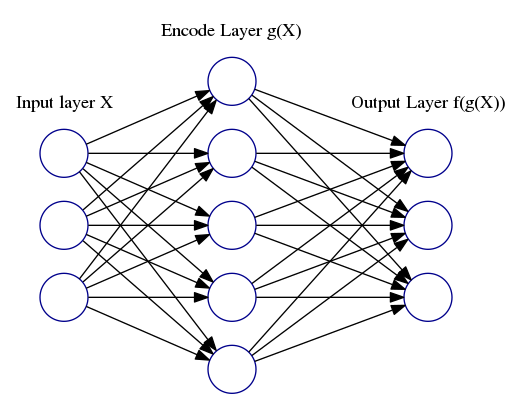
\includegraphics{parts/res/autoencoder.png}}
  } 
  \caption{Auto-Encoder}
  \label{fig:autoenc}
\end{figure} 
\subsection{\label{seq:DeepClust}Deep Clustering}
A several approaches for the deep $K$-Means propose to jointly learn the
representation and perform the $K$-Means algorithm \cite{2018arXiv180107648A}.
In these approaches, network's loss is divided in two parts :
The non-clustering loss does not
take into account of the clustering parts. In general, the non-clustering 
loss is the reconstruction loss of the auto-encoder. We can add additional 
information in the non-clustering loss to bias the representation. For
example, in our case, we add penalties to integrate lexical constraints
.
The clustering loss allows to learn a  $K$-means friendly representation.
Moradi Fard, Thonet and Gaussier \cite{Deap-K-Means} proposed a method for deep $K$-Means 
clustering based on a continuous reparametrization of the objective function 
that leads to a truly joint solution. 
The problem takes the form : 
\begin{equation}
\begin{array}{ll}
L(C ,\alpha;\theta,R) = & \sum\limits_{X \in C} ||X - A(X;\theta)||_2^2 \\
  & + \lambda_0 \sum\limits_{X \in C}||h_\theta(X) - c(h_\theta(X); R) ||_2^2
\end{array}
\end{equation}
where $c(g(X; \theta); R) = \argmin\limits_{k = 1 .. K} || h_\theta(X) - r_k||_2^2$
is a non differentiable function that assigns the document X
to its nearest centroid.\\
They transform this representation as follows :
\begin{equation}
\begin{array}{ll}
L(C ,\alpha;\theta,R) = & \sum\limits_{X \in C} ||X - A(h_\theta(X))||_2^2 + \\ 
& \lambda_0 \sum\limits_{X \in C}\sum\limits_{k=1}^K||h_\theta(X) - r_k ||_2^2 G_{k}(h_\theta(X), \alpha; R) 
\end{array}
\end{equation}
where $G_{k}$ is a differentiable function such that :
\begin{equation}
  \lim\limits_{\alpha \rightarrow \alpha_0}G_{k}(h_\theta(X), \alpha; R) = \left\{
\begin{array}{ll}
  1 & \mbox{if} r_k = c(h_\theta(X); R)\\
  0 & \mbox{Otherwise.}
\end{array}
\right.
\end{equation}
where $\alpha$ play the role of an inverse temperature. In \cite{Deap-K-Means}
, $G_{k}$ was chosen to be a parameterized softmax : 
$G_{k}(h_\theta(X), \alpha; R) = \frac{e^{-\alpha F(h_\theta(X),r_k)}}
{\sum\limits_{k' = 1}^K e^{-\alpha F(h_\theta(X),r_k')}}$\\
To update $(\theta, R)$, they used the stochastic gradient descent (SGD)
as follows :
\begin{equation}
  (\theta, R) \gets (\theta, R) - \epsilon \frac{1}{|\widetilde{C}|}
  \nabla_{(\theta, R)} L(C, \alpha; \theta, R)
\end{equation}
where $\widetilde{C}$ is a random mini batch of C, and $\epsilon$ the
learning rate.
Algorithm \ref{algo:dkm} summarizes the deep k-Means algorithm :
\begin{algorithm}[!h]
  \SetKwInOut{Input}{input}
  \SetKwInOut{Output}{output}
  \Input{Corpus C , number of clusters K, balancing parameter $\lambda_0$,
    scheme for $\alpha$, number of epochs T ,
    number of minibatches MB , learning rate $\epsilon$}
  \Output{Auto-Encoder parameter $\theta$, cluster representative R}
  Initialize $\theta$ and $r_k$, $1 \leq k \leq K$ (randomly or through 
  pretraining)\\
  \ForEach{$\alpha = m_\alpha : M_\alpha$}{
    \ForEach{t = 1 : T}{
      \ForEach{n = 1 : MB}{
        Draw minibatch $\widetilde{C} \subseteq  C$\\
        Update ($\theta, R$) using SGD
      } 
    }  
  }
  \caption{\label{algo:dkm}Deep $K$-Means}
\end{algorithm}
\subsection{\label{seq:BackLexicalConstraint}Lexical Constrain}
Li, Xing, Sun and Ma \cite{Li:2016:EDL:2983323.2983721} proposed a
classification algorithm using Keywords. They assume that keywords could be 
semantically or statistically related to the seed words of the same category.
In this paper, they
use a function $p$ to compute the co-occurrence of each word of a document
with keywords of each categories : 
\begin{equation}\label{sim}
p(i|w) = \frac{df(w,i)}{df(w)}
\end{equation}
where $df(w)$ is the number of the documents containing keywords $w$,
$df(w, i)$ is the number of the documents containing both word
$i$ and keywords $w$.
Then, they calculate the relevance score $rel(i, k)$ for each 
word i and category k as follows :
\begin{equation}\label{rel}
  rel(i,k) = \frac{1}{|k|} \sum\limits_{w \in k} s(w,i)
\end{equation}
\begin{equation}\label{nu}
  \nu(i,k) = max \left(\frac{rel(i,k)}{\sum\limits_{k' \in KW}rel(i,k')} - \frac{1}{|KW|}, 0\right)
\end{equation}
In Equation \ref{nu}, they normalize the relevance score $rel(i,k)$ and 
subtract it by the average relevance score for each category. It is
expected that word $i$ is a category word for category $k$ only if $i$ and
$k$ have a high $rel(i,k)$ value. Therefore subtracting the relevance
scores by the average is necessary to filter out irrelevant categories.